\documentclass[11pt]{article}
\usepackage{appendix}
\usepackage{graphicx} 
\usepackage{setspace}
\usepackage{amsmath,float,verbatim,multicol}
\usepackage{array}
\usepackage{lscape}
\usepackage{hyperref}

\usepackage{amssymb}
\bibliographystyle{plainnat}
\usepackage[round]{natbib}
\usepackage{multirow}

\setlength{\textheight}{8.8in} \setlength{\textwidth}{6.3in}
\setlength{\oddsidemargin}{0.2in} \setlength{\topmargin}{-0.30in}
\setlength{\footnotesep}{10.0pt}

\newcommand{\ol}{\overline}



\renewcommand{\baselinestretch}{1.25}
\title{Quadratic Menu Costs with Reinforcement Learning  }
\author{ Trevor Gallen \\ Econ 64200 }
\date{Fall 2023}

\begin{document}
\bibliographystyle{myplainnat}
%\bibpunct{(}{)}{;}{a}{}{,}6868

\maketitle

This homework asks you to write down and run a simple dynamic problem using reinforcement learning.
\textbf{Deliverables}
\begin{itemize}
\item You should have a word/\LaTeX document that has three sections: 
\begin{enumerate}
\item Discusses the model and answers the questions I pose throughout.
\item Contains the tables and figures you will produce.
\item Contains a discussion of your programming choices if you had to make any.
\end{enumerate}
\item You should have a Matlab file or set of files (zipped) that contain \textbf{all} your programs and raw data.  There should be a file called ``Main.M" that produces everything I need in one click.
\end{itemize}


\section{Model}
Each period, firms begin the period with prices $p_{t-1}$ and observe optimal price $\overline{P}_t$.  They may either change their price $p_t$, which costs $\phi(p_{t}-p_{t-1})^2$, or leave it fixed at $p_{t-1}$.  Their value function is:
$$V(p_{t-1},\overline{P}_t)=\underset{p_t}{\max} -(p_t-\overline{P}_t)^2-\phi(p_{t}-p_{t-1})^2+\beta V(p_{t},\overline{P}_{t+1})$$
Where:
$$\overline{P}_t=\rho \overline{P}_{t-1}+\epsilon\ \ \ \epsilon\sim\mathcal{N}\left(0,\sigma^2\right)$$
Let $\rho=0.95$, $\sigma=0.01$, and $\phi=0.1$.  Discount factor is 0.95.
\ \\
\ \\

\section{Problems}
\textbf{Question 1} Do the following in matlab:
\begin{itemize}
\item Define an environment for the problem: observation (2x1) and action info (1x1).
\item Write out a reset function for state variables $p_{t-1}$ and $\overline{P}_t$
\item Write out a step function that takes in $\overline{P}_t$, $p_{t-1}$ and $p_{t}$ and generates the reward and next  $\overline{P}_{t+1}$
\item Define a critic network, and actor network, and an agent
\item Train the agent
\item Display the agent's optimal policy function for $p_t$ as a function of $\overline{P}_t$ and $p_{t-1}$.
\end{itemize}
 
 \textbf{Suggested Solutions}:\\
 \ \\
 See Main.m.  I solved this with value function iteration as well as reinforcement learning to compare.  If you examine the VFI solutions, you find that the simple linear policy function that summarizes most of the true policy function is to set $p_t=0.91 \overline{P}_t+0.09 p_t$.  \\
 \ \\
With that in mind (when it comes to RL, it's useful to give all the correct information you can--nonparametric learning is hard!) I used a fairly simple neural network for the actor with two hidden+ReLU layers, each of breadth of 10. For the critic, I had a hidden layer+ReLU after the observation as well as action (each 20) then combined those outputs (layer is 40) and did two more hidden layers+ReLU until a final output layer.\\
\ \\
To make things converge rapidly, I first only fed in 7,000 iterations of maximum length 3.  Note that this isn't like having the agent ``die" after three periods, because the algorithm fills in the no-end-period-but-end-of-data with the value function + the next state, so this could actually be sufficient to converge to the policy function.  However, it wouldn't converge to the Q/value function's level, because it has a maximum horizon of three.\\
\ \\
To try to get the level, I then fed it 200 periods.\\
\ \\
I plot both the VFI and RL value functions (critic+actor's action gives value function) in Figure 1, along with their policy functions.  You can see that the policy functions are mostly spot on, though at the edges (where the RL agent it less likely to learn) there is curvature not present in VFI.  I could probably overcome this by setting the initial conditions to more heavily emphasize the outside possibilities and having a more complicated (either breadth or depth) function.\\
\ \\
Finally, note that I have a ``policy function iteration" like possibility in my code.  If you turn \texttt{pretrain = 1} on, then I first simulate the value and actor if the agent first chooses a random action (for the Q-function) and then chooses $p_t=\bar{P}_t$ from then on.  This is not the optimal policy, but will give the broad shape of the Q-function.\\
\ \\
To ``pre-train" my neural networks, I add a regression layer to each, and feed my simulated data to the critic (state draw+action draw+realized value) and the actor (state draw+action draw).  These give something pretty near the actual VFI shape, and converges \emph{much much} faster than going in na\"{\i}vely.  

\begin{figure}
\centering
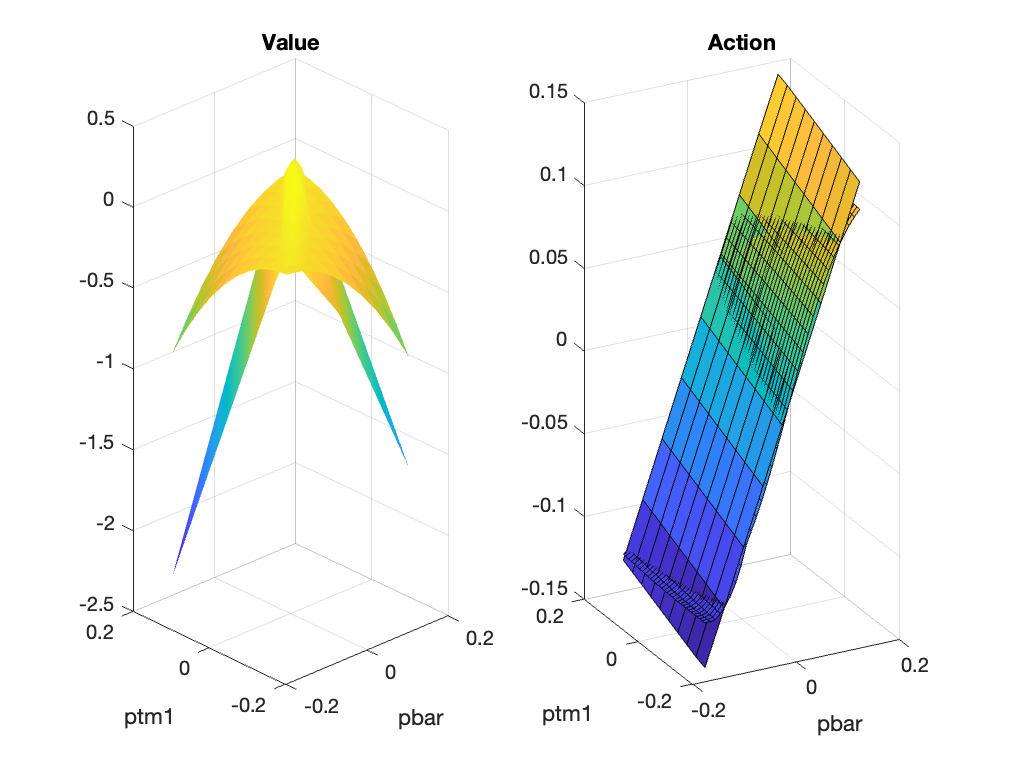
\includegraphics[scale=0.5]{Value_and_Action.png}
\caption{The left hand figures show the VFI value function and the RL value function.  The RL value function is the ``sharp" value function while the ``true" VFI value function is far shallower.  The right hand figure is the two policy functions, which are mostly right on top of one another, save at the edges.}
\end{figure}

\end{document}





